\label{sec:Preproc}
In this section we consider the problem of designing a feedforward controller. Such a problem may arise if there is no feedback signal, or if we wish to use a preview precompensator to enhance an existing feedback controller. 

It follows from (\ref{proj_prop}) and the fact that a feedforward controller does not alter $T_{w\rightarrow z}$, that $\nrm{T_{\tiny{\ma{w\\ \eta}\rightarrow z}}}_2$ is minimised by choosing the feedforward controller which minimises $\nrm{T_{\eta \rightarrow z}}_2$. Given these observations, we may neglect the influence of $w$ in the design process.

\begin{figure}
\begin{center}
\stdcontrolfrags
\psfrag{rhat}{}
\psfrag{KFF}{$K_{FF}$}
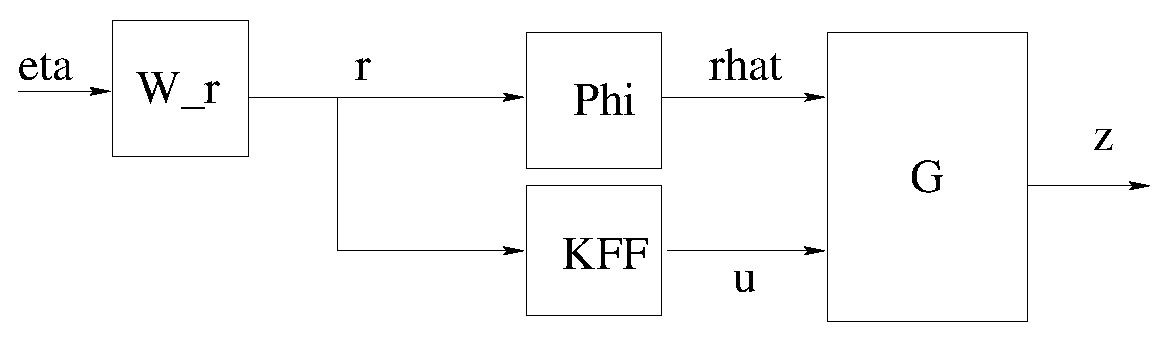
\includegraphics[width=9cm]{./diags/DistRejSysFF.eps}
\end{center}
\caption{A feedforward controller design problem. The notation follows that of Figure \ref{fig:DistRejSys}.\label{fig:DistRejSysFF}}
\end{figure}

The problem considered in this section is illustrated in Figure \ref{fig:DistRejSysFF}. By modifying (\ref{eqn:P}), it follows that the appropriate generalised plant is given by:
\aln{
P_{FF}&\shorteq\ma{\arr{cc|c:c}{
A_g&B_{1gr}C_{d1}&0&B_{2g}\\
0&A_d&B_{d}&0\\\hline
C_{1g} &D_{11gr}C_{d1} &0&D_{12}\\ \hdashline
0&C_{d2}&D_r&0
}}\label{eqn:PFF}\\
&=\ssmod{A}{B_1}{B_2}{C_1}{C_2}{D_{11}}{D_{12}}{D_{21}}{0}
.}

It is easily checked that the associated full-information control is obtained by removing the gain associated with $w$, and so  $K_{FI}=\ma{F_{2g} &F_{2p}&F_{2r} & F_{0r} }$, where the gains may be computed using (\ref{eqn:F2g}) and (\ref{eqn:F2pEff})-(\ref{eqn:F0reff}). To arrive at this result one need only retrace the derivations of Section \ref{sec:H2FI}, with $B_{1gw}$ and $D_{11gw}$ set to zero.

Next, we give a result concerning the solution to the estimation DARE:
\begin{lem}
If $A_g$ is stable and $W_r$ is outer, then the version of the DARE (\ref{eqn:Y2d}) associated with (\ref{eqn:PFF}) has a stabilising solution $Y=0$.
\end{lem}
\begin{proof}
First note that if $Y=0$, then:
\als{
L_2&= -\ma{0\\B_dD_r^{-1}}\\
\bar S&= D_rD_r'
,}
from which it can be checked that $Y=0$ solves (\ref{eqn:Y2d}). This solution is stabilising because:
\als{
A+L_2C_2=\ma{A_g &B_{1gr}C_{d1}\\0&A_d-B_dD_r^{-1}C_{d2}  }
}
is stable since $A_g$ is stable and $W_r$ is outer (see (\ref{eqn:AdBdDrCd2})).
\end{proof}
If we also note that:
\als{L_0&= F_{0r}D_r^{-1},}
with $F_{0r}$ defined in (\ref{eqn:F0reff}),
then we can use (\ref{eqn:H2OptK}) to obtain the following $\htwo$-optimal controller:
\als{
K_{FF}& \shorteq \ma{\arr{c|c}{A_K&B_K\\\hline C_K&D_K}}\\
A_K&=\ma{A_g+B_{2g}F_{2g}&B_{1gr}C_p+B_{2g}F_{2p}&B_{2g}F_{2r}-B_{2g}F_{0r}D_r^{-1}C_r\\
0&A_p&0\\
0&0&A_r-B_rD_r^{-1}C_r}\\
B_K&=\ma{B_{2g}F_{0r}D_r^{-1}\\
	B_p\\
	B_rD_r^{-1}}\\
C_K&=\ma{F_{2g}&F_{2p}&F_{2r}-F_{0r}D_r^{-1}C_r}\\
D_K&=F_{0r}D_r^{-1}
,}
%
which has the low order representation:
\als{
\bar K_{FF} \shorteq \ma{\arr{cc|cc}{
A_g+B_{2g}F_{2g}&B_{2g}F_{2r}-B_{2g}F_{0r}D_r^{-1}C_r  & B_{1gr}C_p+B_{2g}F_{2p} & B_{2g}F_{0r}D_r^{-1}\\
0 & A_r-B_rD_r^{-1}C_r & 0 & B_rD_r^{-1}\\\hline
F_{2g} & F_{2r}-F_{0r}D_r^{-1}C_r & F_{2p} & F_{0r}D_r^{-1}
}}}
%
such that the optimal control is given by:
\als{
u^*&=\bar K_{FF} \bar r
}
in which
\als{
\bar r(k)&=\ma{r(k-N)\\\vdots\\r(k)}.
}
